% ======================================================================
%  Compile with pdflatex.
% ======================================================================
\documentclass[twoside,leqno,twocolumn]{article}  
\usepackage[nocopyright,siamsections,siamtitle,smallbib]{jeffeproc} 

%page dimensions from ltexpprt.sty
%\pretolerance=800 
%\tolerance=10000 
%\sloppy 
%\vsize=55pc 
%\hsize=41pc 
%\baselineskip=14pt 
%\footskip=18pt 
\topmargin -24pt  
\headheight 12pt  
\headsep 17pt  
\parskip 1pt plus 1pt minus 1pt
\parindent 1.5em
\textheight 52.5pc  \advance\textheight by \topskip 
\textwidth 41pc  
\setlength{\oddsidemargin}{-0.875pc} 
\setlength{\evensidemargin}{-0.875pc}

\usepackage{jeffe,graphicx,hyperref}
\usepackage{marvosym}
\usepackage[utf8]{inputenc}

\clubpenalty 10000
\widowpenalty 10000

%-----------------------------------------------------------------------
%  These packages are purely cosmetic.
%  Just comment them out if they don't work for you.
%-----------------------------------------------------------------------
\usepackage{microtype}
\usepackage[charter]{mathdesign}
\def\sfdefault{fvs}
\def\ttdefault{fvm}
\usepackage[mathcal]{euscript}
\usepackage{stmaryrd}


%-----------------------------------------------------------------------
%  Local definitions
%-----------------------------------------------------------------------
\def\arcto{\mathord\shortrightarrow}
\def\arc#1#2{#1\arcto#2}
\def\cra#1#2{#1\mathord\shortleftarrow#2}
\def\fence#1#2{#1\mathord\shortuparrow#2}
\def\ecnef#1#2{#1\mathord\shortdownarrow#2}
\def\head{\mathit{head}}
\def\tail{\mathit{tail}}
\def\lsh{\mathit{left}}
\def\rsh{\mathit{right}}
\def\rev{\mathit{rev}}
\def\Z{\mathbb{Z}}
\def\Real{\mathbb{R}}
\def\Q{\mathbb{Q}}

% needs marvosym package:
\def\snip{\mathbin{\raisebox{0.15ex}{\rotatebox[origin=c]{60}{\Rightscissors}\!}}}
\let\unlhd\trianglelefteq	% fix mathdesign font bug

\let\cycle\gamma
\let\path p
\let\primalarc\alpha
\def\dualarc{p}

\def\Sigmabar{\overline{\smash{\Sigma}\vphantom{t}}}
\def\SIGMABAR{\boldsymbol{\overline{\smash{\Sigma}\vphantom{x}}}}
\def\Gbar{\overline{\smash{G}\vphantom{t}}}
\def\Vbar{\overline{\smash{V}\vphantom{t}}}
\def\Ebar{\overline{\smash{E}\vphantom{t}}}
\def\bbar{\overline{\smash{b}\vphantom{t}}}
\def\nbar{\overline{n}}
\def\gbar{\overline{g}}
\def\wbar{\overline{w}}
\def\sigmabar{\overline{\sigma}}
\def\cyclebar{\overline{\cycle}}
\def\chibar{\overline{\chi}}

\def\fakeparagraph#1{\par\medskip\noindent\textbf{#1}}


\newtheorem{theorem}{Theorem}[section]
\newtheorem{corollary}[theorem]{Corollary}
\newtheorem{lemma}[theorem]{Lemma}


%\pagestyle{myheadings}
%\markboth{Computing Replacement Paths in Surface Embedded Graphs}
%		 {Jeff Erickson and Amir Nayyeri}
\pagestyle{empty}

\urldef\paperURL\url{http://www.cs.uiuc.edu/~jeffe/pubs/homcover.html}


% --------------------------------------------------------------------------------
\begin{document}


\title{Minimum Cuts and Shortest Non-Separating Cycles\\
	 via Homology Covers%
\thanks{This research was partially supported by NSF grant CCF 09-15519.  See \paperURL\ for the most recent version of this paper.}}

\author{
	Jeff Erickson\\[1ex]
	\normalsize
	\begin{tabular}{c}
	Department of Computer Science\\
	University of Illinois at Urbana-Champaign\\
	\protect\url{jeffe@cs.uiuc.edu}
	\end{tabular}
	\and
	Amir Nayyeri	\\[1ex]
	\normalsize
	\begin{tabular}{c}
	Department of Computer Science\\
	University of Illinois at Urbana-Champaign\\
	\protect\url{nayyeri2@cs.uiuc.edu}
	\end{tabular}
}

%\date{Submitted to SODA 2011 --- \today}

\maketitle


\begin{abstract}
Let $G$ be a directed graph with weighted edges, embedded on a surface of genus~$g$.  We describe an algorithm to compute a shortest directed cycle in $G$ in any given $\Z_2$-homology class in $2^{O(g)}n\log n$ time; this problem is {NP}-hard even for undirected graphs.  We also present two applications of our algorithm.  The first is an algorithm to compute a shortest non-separating directed cycle in $G$ in $2^{O(g)} n\log n$ time, improving the recent algorithm of Cabello \etal\ [SOCG 2010] for all $g=o(\log n)$.  The second is a combinatorial algorithm to compute minimum $(s,t)$-cuts in \emph{undirected} surface graphs in $2^{O(g)} n\log n$ time, improving on previous combinatorial algorithms, and in particular the recent  of Chambers \etal\ [SOCG 2009], for all~$g = o(\log n)$.  Unlike earlier algorithms for surface graphs that construct and search finite portions of the universal cover, our algorithms use another canonical covering space, called  the \emph{$\Z_2$-homology cover}.
\end{abstract}


% --------------------------------------------------------------------------------
\section{Introduction}

Algorithms to find optimal subgraphs with certain properties in surface-embedded graphs are a basic ingredient in numerous algorithms in topological graph theory.  Structures of interest include minimum spanning trees, single- and multiple-source shortest paths \cite{cc-msspg-07, multishort, hkrs-fspap-97, k-msspp-05}, minimum cuts \cite{surfcut, surflow}, shortest topologically interesting cycles \cite{c-mdpg-06, multishort, ccl-fsncd-10, schema, k-csnco-06, t-egnsn-90}, shortest paths or cycles homotopic to a given path or cycle \cite{cl-opdsh-07, octagons, hs-cmlpg-94}, shortest cut graphs \cite{c-scgsp-10, schema, gohog}, and shortest generators for homotopy or homology groups \cite{dls-chtl-07, gohog}.  Applications of these basic algorithms include probabilistically embedding high-genus graphs into planar graphs \cite{bls-rrgh-09,ls-ggcg-10,s-osp-10}, drawing abstract graphs in the plane with the fewest possible crossings~\cite{kr-ccnlt-07}, testing isomorphism between graphs of fixed genus \cite{km-gmiap-08}, approximating optimal traveling salesman tours~\cite{dhm-aacd-07} and Steiner trees~\cite{bdt-ptass-08, bkk-ptass-07, bkk-stpg-07}, and computing low-distortion surface parametrizations \cite{ssp-cetm-08, tacd-dqdhf-06}.

In this paper, we describe an algorithm to compute a shortest \emph{directed} cycle in a specified $\Z_2$-homology class, in a \emph{directed} $n$-vertex graph embedded on a surface of genus $g$, in $2^{O(g)}n\log n$ time.  (See Section \ref{S:back} for a brief overview of $\Z_2$-homology.)   We are unaware of any previously published algorithm for this problem; however, an algorithm of Chambers \etal~\cite{splitting} can be modified to find shortest homologous cycles in \emph{undirected} graphs in $g^{O(g)} n\log n$ time.  This problem can be shown to be {NP}-hard, even for undirected graphs, by a reduction from the traveling salesman problem in grid graphs~\cite{splitting}.

We also describe two applications of our main result.  As an immediate corollary, we obtain an algorithm to compute a shortest non-separating cycle in a surface-embedded directed graph in $2^{O(g)} n\log n$ time (Corollary~\ref{C:nonsep}).  Although the corresponding problem in undirected graphs is well studied, the first nontrivial results for directed graphs were only recently published by Cabello \etal~\cite{ccl-fsncd-10}, who describe an algorithm that runs in $O(g^{1/2} n^{3/2}\log n)$ time.  Our algorithm is faster when $g=o(\log n)$.

Our second application (Section \ref{S:mincut}) is a combinatorial algorithm to compute minimum $(s,t)$-cuts in \emph{undirected} surface graphs in $2^{O(g)} n\log n$ time.  Like Chambers \etal~\cite{surfcut}, we reduce the minimum cut problem to the more general (and {NP}-hard) problem of computing a minimum-cost \emph{subgraph} in any given $\Z_2$-homology class.  We solve this more general problem by combining our algorithm to find minimum \emph{cycles} in each homology class with a straightforward dynamic programming algorithm.  The resulting algorithm is both simpler and faster  than the minimum-cut algorithm of Chambers \etal~\cite{surfcut}, which runs in $g^{O(g)} n\log n$ time.  When $g = o(\log n)$, our algorithm is also faster than the best combinatorial minimum-cut algorithms for arbitrary sparse graphs, which run in $O(n^2\log n)$ time~\cite{st-dsdt-83, gt-namfp-88}.

Many previous algorithms for finding optimal substructures are based on a common approach, first suggested by Kutz \cite{k-csnco-06}.  An exchange argument implies an upper bound on the number of times that the target structure can cross a shortest path; for example, the shortest non-separating cycle intersects any shortest path at most once~\cite{cm-fsnsn-07}.  Ultimately, this crossing bound follows from the observation that two shortest paths in a generic undirected surface graph cross at most once.  The crossing bound implies that the target structure lies in one of a finite number of \emph{homotopy} classes.  (See Section~\ref{S:back} for definitions.)  For each candidate homotopy class, these algorithms construct and search a relevant finite portion of the (infinite) universal cover of the input surface, using planar shortest-path algorithms \cite{hkrs-fspap-97, k-msspp-05}.

For directed surface graphs, however, this approach appears doomed from the start.  Two \emph{directed} shortest paths can cross arbitrarily many times; similarly, a shortest non-separating directed cycle can cross a directed shortest path arbitrarily many times.  Even for undirected graphs, finding optimal cycles in a given \emph{homology} class by enumerating \emph{homotopy} classes seems unnecessarily baroque.  In this paper, we abandon crossing bounds and homotopy methods entirely, and work directly with homology instead, at every stage of our algorithm and its analysis.  Instead of the universal cover, our algorithms construct and search another canonical covering space, called the \emph{$\Z_2$-homology cover}, which we describe in detail in Section \ref{S:cover}.  We also use a recent generalization of Klein's seminal multiple-source shortest path algorithm~\cite{k-msspp-05} to higher-genus embedded graphs \cite{cc-msspg-07,multishort}.

\subsection{Related Results}

\textbf{Minimum cuts.~}
Minimum cuts and maximum flows have been studied in planar graphs for more than half a century, starting with the seminal work of Ford and Fulkerson \cite{ff-mfn-56} and others \cite{hr-fmern-55}.  A long series of results eventually led to an algorithm by Reif~\cite{r-mstcp-83} to compute minimum $(s,t)$-cuts in \emph{undirected} planar networks in near-linear time; Frederickson~\cite{f-faspp-87} later improved the running time of Reif's algorithm to $O(n\log n)$.  The only efficient method known to compute minimum cuts in \emph{directed} planar graphs is to compute a maximum flow~\cite{w-mstfp-97, bk-amfdp-09, parshort}.  Janiga and Koubek described an adaptation of Reif's algorithm, to \emph{directed} planar networks in near-linear time \cite{jk-mcdpn-92}; however, their algorithm has a subtle error \cite{n-pc-10}.

Surprisingly little is known about computing minimum cuts in natural generalizations of planar graphs.  Chambers~\etal~\cite{surfcut} described an algorithm to compute a minimum $(s,t)$-cut in an \emph{undirected} graph embedded on a surface of genus $g$, for any specified vertices $s$ and~$t$, in $g^{O(g)}n\log n$ time.  The fastest algorithm to compute minimum $(s,t)$-cuts in  directed surface graphs, also due to Chambers~\etal~\cite{surflow}, computes a maximum $(s,t)$-flow in near-linear time for graphs of constant genus and polynomially-bounded capacities.

\fakeparagraph{Shortest non-trivial cycles.~}
The problem of finding shortest topologically nontrivial cycles in embedded \emph{undirected} graphs has a long history.  Itai and Shiloach \cite{is-mfpn-79} observed that the minimum $(s,t)$-cut in an undirected planar graph~$G$ is dual to the minimum-cost cycle that separates faces $s^*$ and $t^*$ in the dual graph~$G^*$.  Thus, Frederickson's minimum cut algorithm~\cite{f-faspp-87} computes the shortest nontrivial cycle in a combinatorial annulus in $O(n\log n)$ time.  Thomassen \cite{t-egnsn-90} developed the first efficient algorithm for graphs on arbitrary surfaces, which runs in $O(n^3)$ time and exploits the so-called \emph{3-path condition}; see also Mohar and Thomassen~\cite[Sect.~4.3]{mt-gs-01}.  Erickson and Har-Peled described a faster algorithm that runs in $O(n^2 \log n)$ time \cite{schema}.  This is the fastest algorithm known for arbitrary surface-embedded graphs; however, several faster algorithms are known when the genus $g$ of the underlying surface is small \cite{cm-fsnsn-07, c-mdpg-06, k-csnco-06, cc-msspg-07, multishort}.  For related results, see \cite{ccl-osaew-10,tight,splitting,essential}.

The history for \emph{directed} embedded graphs is much shorter, in part because neither Thomassen's 3-path condition nor Cabello and Mohar's crossing condition hold.  The shortest nontrivial \emph{directed} cycle in an annular graph is dual to either the minimum $(s,t)$-cut or the minimum $(t,s)$-cut in the directed planar dual graph, whichever has smaller capacity.  Both of these cuts can be computed in $O(n\log n)$ time using planar flow algorithms.\footnote{It appears that Jeniga and Koubeck's algorithm \cite{jk-mcdpn-92} always correctly computes the smaller of these two cuts.}  Very recently, Cabello \etal~\cite{ccl-fsncd-10} describe an algorithm to find a shortest non-contractible or non-separating cycle in a directed surface graph in  $O(\sqrt{g}n^{3/2}\log n)$ time, using a subtle generalization of Thomassen's 3-path condition.

\fakeparagraph{Shortest equivalent cycles.~}
Several authors have considered the related question of finding the shortest cycle in a surface graph that is either homotopic or homologous to a given cycle.  Colin de Verdière and Erickson \cite{octagons} describe an algorithm to compute the shortest cycle homotopic to a given cycle in a combinatorial surface in $O(gnk \log nk)$ time, where $k$ is the number of edges in the input cycle, improving and generalizing previous results of Colin de Verdière and Lazarus for \emph{simple} cycles~\cite{cl-opdsh-07}.  An argument of Chambers \etal~\cite{splitting} implies that finding the shortest cycle (either simple or not) in a given \emph{homology} class in a surface graph is NP-hard; Chen and Friedman \cite{cf-qhc-08,cf-hrhl-10} proved that the corresponding problem in simplicial complexes is NP-hard to approximate within any constant factor.

The minimum-cut algorithm of Chambers \etal~\cite{surfcut} can be used to compute the minimum-cost \emph{even subgraph} in a given $\Z_2$-homology class in $g^{O(g)}n\log n$ time; this problem is also NP-hard in general.  Chambers \etal~\cite{surflow} described algorithms to find the minimum-cost \emph{circulation} in a given real or integer homology class in a directed surface-embedded graph in polynomial time; Dey \etal~\cite{dhk-ohctu-10} generalized this result to arbitrary chains of arbitrary dimension in arbitrary simplicial complexes.  For other related results, see \cite{cf-mcngh-10,dls-chtl-07,gohog,zc-lh-07}.

% --------------------------------------------------------------------------------
\section{Notation and Terminology}
\label{S:back}

We begin by recalling several useful definitions related to surface-embedded graphs.  For further background, we refer the reader to Gross and Tucker \cite{gt-tgt-01} or Mohar and Thomassen~\cite{mt-gs-01} for topological graph theory, and to Hatcher~\cite{h-at-01} or Stillwell~\cite{s-ctcgt-93} for surface topology and homology.

\fakeparagraph{Surfaces and curves.~}
A \EMPH{surface} (more formally, a \emph{2-manifold with boundary}) $\Sigma$ is a compact Hausdorff space in which every point has an open neighborhood homeomorphic to either the plane $\Real^2$ or a closed halfplane $\set{(x,y)\in \Real^2\mid x\ge 0}$.  The points with halfplane neighborhoods make up the \EMPH{boundary} of $\Sigma$; the complement of the boundary is the \EMPH{interior} of $\Sigma$.  Every component of the boundary is homeomorphic to a circle.  A surface is \emph{non-orientable} if it contains a subset homeomorphic to the \Mobius\ band, and \emph{orientable} otherwise.

A \EMPH{path} in a surface $\Sigma$ is a continuous function $p\colon [0,1]\to\Sigma$.  A \EMPH{loop} is a path whose endpoints $p(0)$ and $p(1)$ coincide; we refer to this common endpoint as the \EMPH{basepoint} of the loop.  An \EMPH{arc} is a path whose endpoints lie on the boundary of $\Sigma$.  A \EMPH{cycle} is a continuous function $\gamma\colon S^1\to\Sigma$; the only difference between a cycle and a loop is that a loop has a distinguished basepoint.  We collectively refer to paths, loops, arcs, and cycles as \EMPH{curves}.  A curve is \EMPH{simple} if it is injective, except for the basepoint in the case of loops; we usually do not distinguish between simple curves and their images in $\Sigma$.  The \EMPH{reversal $\rev(p)$} of a path $p$ is defined by setting $\rev(p)(t) = p(1-t)$.  The \EMPH{concatenation $p \cdot q$} of two paths $p$ and $q$ with $p(1) = q(0)$ is the path created by setting $(p\cdot q)(t) = p(2t)$ for all $t \le 1/2$ and $(p\cdot q)(t) = q(2t-1)$ for all $t \ge 1/2$.

The \EMPH{genus} of a surface $\Sigma$ is the maximum number of disjoint simple cycles $\gamma_1, \gamma_2, \dots, \gamma_g$ in the interior of $\Sigma$ whose complement $\Sigma\setminus(\gamma_1\cup\cdots\cup\gamma_g)$ is connected.  We will consider only compact, connected, orientable surfaces.  Up to homeomorphism, there is exactly one such surface with any genus $g\ge 0$ and any number of boundary components $b\ge 0$; the \EMPH{Euler characteristic $\chi$} of this surface is $\chi := 2-2g+b$.

\fakeparagraph{Graphs, embeddings, and duality.~}
An \EMPH{embedding} of an undirected graph $G$ on a surface $\Sigma$ maps vertices to distinct points and edges to interior-disjoint curves.  The \emph{faces} of the embedding are maximal connected subsets of $\Sigma$ that are disjoint from the image of the graph.  An embedding is \EMPH{cellular} if each of its faces is homeomorphic to the plane; in particular, in any cellular embedding, each component of the boundary of $\Sigma$ must be covered by a cycle of edges in $G$.  Euler's formula implies that any cellularly embedded graph with $n$ vertices, $m$ edges, and $f$ faces lies on a surface with Euler characteristic $\chi = n-m+f$, which implies that $m = O(n+g)$ and $f=O(n+g)$.  We consider only cellular embeddings of genus $g=O(n)$, so that the overall complexity of the embedding is $O(n)$.

Any undirected graph $G$ embedded on a surface $\Sigma$ with boundary has a \EMPH{dual graph~$G^*$}, defined as follows.\footnote{Our definition differs slightly from the one proposed by Erickson and Colin de Verdi\`ere~\cite{octagons}.}  The dual graph~$G^*$ has a vertex $f^*$ for each face $f$ of~$G$, \emph{including the boundary cycles}, and an edge $e^*$ for each edge $e$ in $G$ (including boundary edges) joining the vertices dual to the faces that $e$ separates.  For each boundary cycle $\delta$ of~$G$, we refer to the corresponding vertex $\delta^*$ of $G^*$ as a \EMPH{dual boundary vertex}.  The dual graph $G^*$ has a natural cellular embedding in the surface~\EMPH{$\Sigma^\bullet$} obtained from $\Sigma$ by gluing a disk to each boundary cycle; each face of this embedding corresponds to a vertex of $G$.  See Figure \ref{F:duality}.  (Duality can be extended to directed graphs~\cite{surflow}, but our results do not require this extension.)

\begin{figure}[htb]
\centering
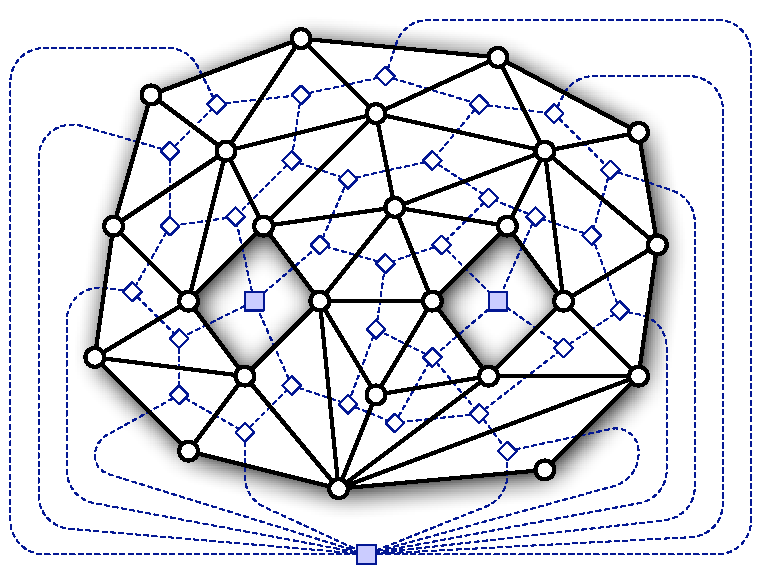
\includegraphics[scale=0.45]{Fig/pants}
\caption{A cellularly embedded graph $G$ (solid lines) on a pair of pants (genus 0 with 3 boundaries), and its dual graph $G^*$ (dashed lines).  Dual boundary vertices are indicated by squares.}
\label{F:duality}
\end{figure}

For any subgraph $F = (U,D)$ of $G = (V,E)$, we write \EMPH{$G\setminus F$} to denote the edge-complement $(V, E\setminus D)$.  Also, when the graph $G$ is fixed, we abuse notation by writing~$F^*$ to denote the subgraph of $G^*$ corresponding to a subgraph $F$ of~$G^*$; each edge in $F^*$ is the dual of a unique edge in~$F$.  In particular, we have the identity $(G\setminus F)^* = G^* \setminus F^*$.

For most of the problems we consider, the input consists of a \emph{directed} edge-weighted graph $G$ with a cellular embedding on some surface.  We use the notation \EMPH{$\arc{u}{v}$} to denote the directed edge from vertex $u$ to vertex $v$.  Without loss of generality, we consider only \emph{symmetric} directed graphs, in which the reversal $\arc{v}{u}$ of any edge $\arc{u}{v}$ is another edge.  We also assume that in the cellular embedding, the images of any edge and its reversal coincide (but with different orientations).  Thus, like Cabello \etal \cite[Section 2.3]{ccl-fsncd-10}, we implicitly model directed graphs as \emph{undirected graphs with asymmetric edge weights}.

Cellular graph embeddings are equivalent to the \EMPH{combinatorial surfaces} introduced by Colin de Verdi\`ere~\cite{c-rcds-03} and used by several authors to formulate optimization problems for surface-embedded graphs.  A~combinatorial surface consists of an abstract surface $\Sigma$ together with a cellularly embedded graph $G$ with (possibly asymmetrically) weighted edges.  Paths and cycles in a combinatorial surface are directed walks in its graph; the length of any such walk is the sum of its (directed) edge weights, counted with appropriate multiplicity.

\fakeparagraph{Homotopy and homology.}
Two paths $\alpha$ and $\beta$ in $\Sigma$ are \emph{homotopic} if one can be continuously deformed into the other.  More formally, a \EMPH{homotopy} between $\alpha$ and $\beta$ is a continuous map $h\colon {[0,1]\times[0,1] \to \Sigma}$ such that $h(0,\cdot) = \alpha$, $h(1,\cdot) = \beta$, $h(\cdot,0) = \alpha(0) = \beta(0)$, and $h(\cdot,1) = \alpha(1) = \beta(1)$.  Homotopy defines an equivalence relation over the set of paths with any fixed pair of endpoints.  The set of homotopy classes of loops in $\Sigma$ with basepoint $x$ defines a group $\pi_i(\Sigma, x)$ under concatenation, called the \emph{fundamental group} of $\Sigma$.  (For all points $x$ and $y$, the groups $\pi_i(\Sigma,x)$ and $\pi_i(\Sigma,y)$ are isomorphic.)

A cycle~$\gamma$ is \emph{contractible} if it is homotopic to a constant map; a simple cycle~$\gamma$ is \EMPH{separating} if $\Sigma\setminus\gamma$ is disconnected.

Homology is a coarser equivalence relation than homotopy, with nicer algebraic properties; intuitively, two cycles are homologous if together they define the boundary of some subset of the surface.  Like several earlier papers \cite{cf-qhc2-07, cf-qhc-08, dls-chtl-07, dlsc-cgaht-08, surfcut}, we will consider only one-dimensional cellular homology with coefficients in the finite field $\Z_2$; this restriction allows us to radically simplify our definitions.  

Fix a cellular embedding of an undirected graph $G$ on a surface $\Sigma$ with genus $g$ and $b$ boundaries.  An \EMPH{even subgraph} is a subgraph of $G$ in which every node has even degree, or equivalently, the union of edge-disjoint cycles.  An even subgraph is \EMPH{null-homologous} if it is the boundary of the union of a subset of faces of $G$.  Two even subgraphs $\eta$ and $\eta'$ are \EMPH{homologous}, or in the same \EMPH{homology class}, if their symmetric difference \EMPH{$\eta\oplus\eta'$} is null-homologous; See Figure \ref{F:homology}.  The set of all homology classes of even subgraphs defines the \EMPH{first homology group} of~$\Sigma$, denoted \EMPH{$H_1(\Sigma; \Z_2)$}, which is isomorphic to the finite vector space $(\Z_2)^\beta$, where $\beta = 2g + \max\set{{b-1}, 0}$.  The rank \EMPH{$\beta$} is called the \EMPH{first Betti number} of~$\Sigma$.

\begin{figure}
\centering
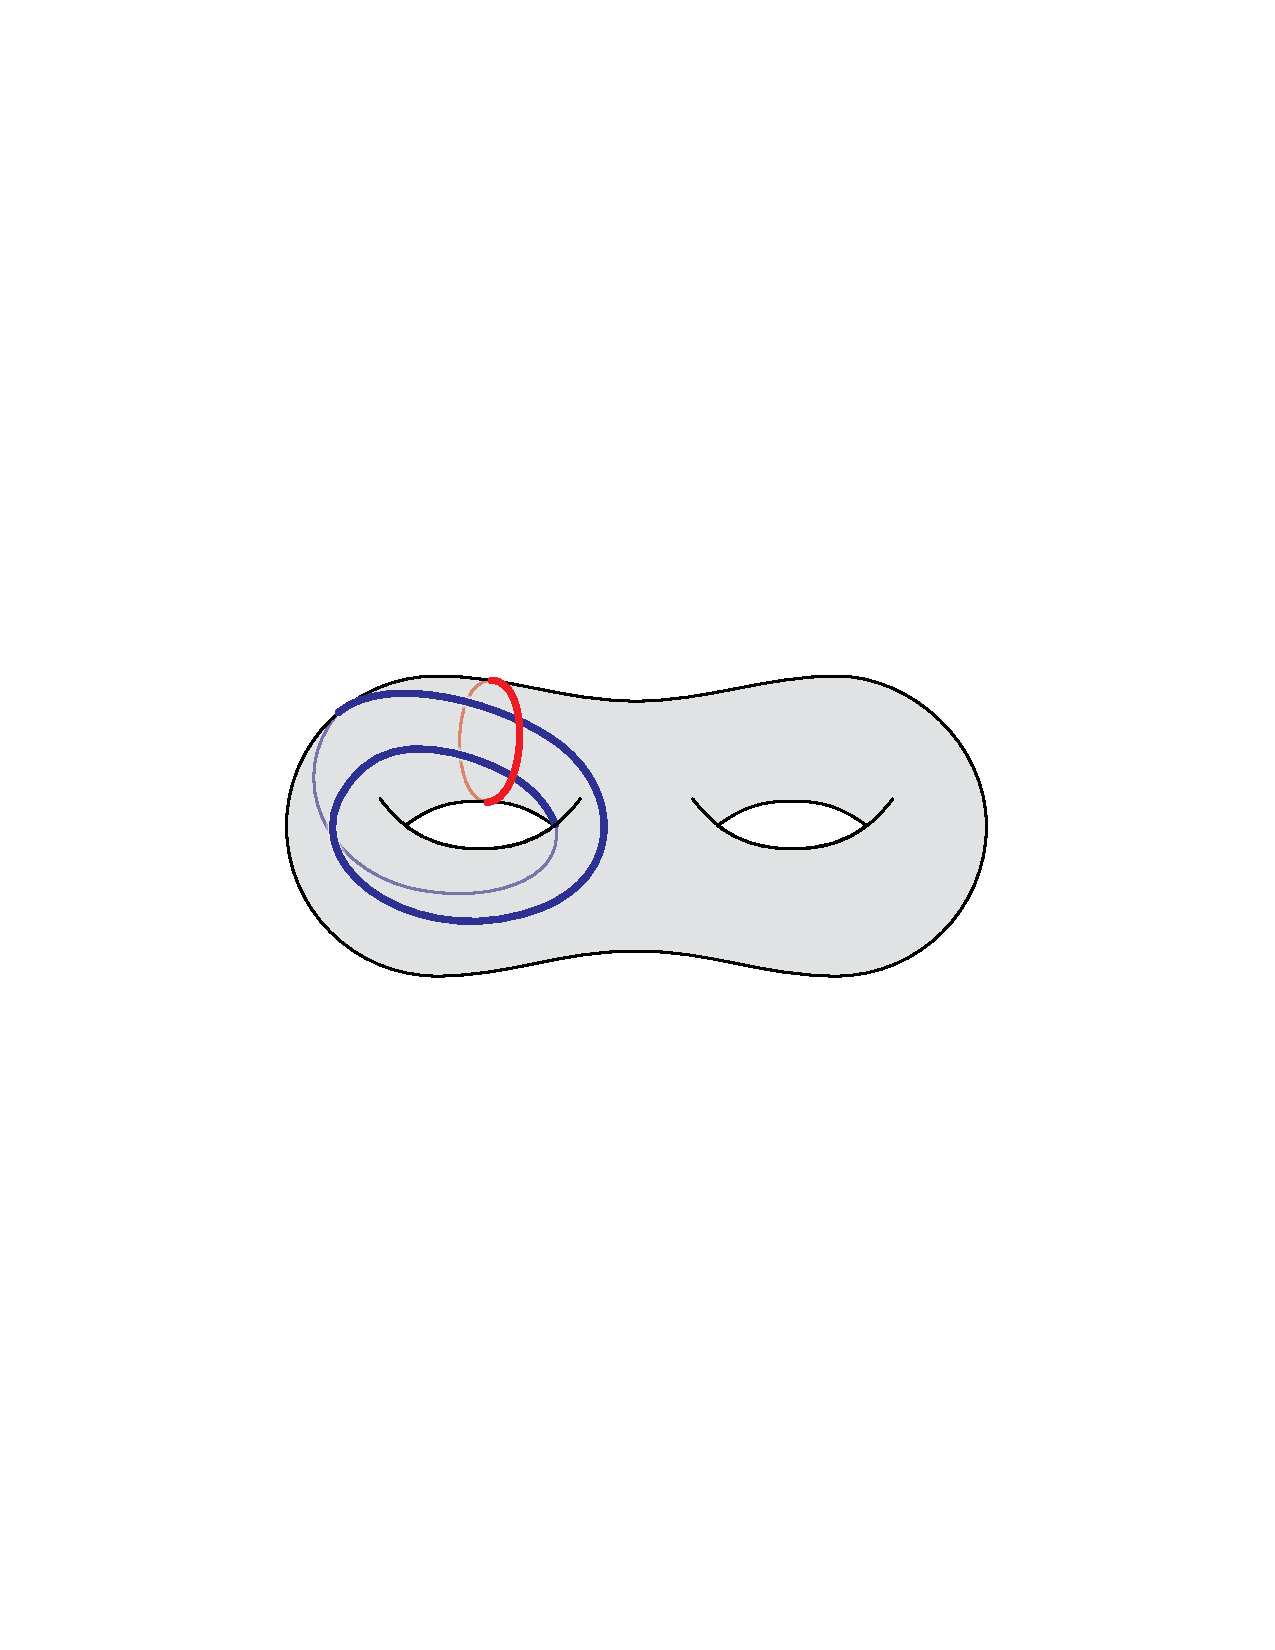
\includegraphics[height=0.75in]{Fig/homologous3}\\[2ex]
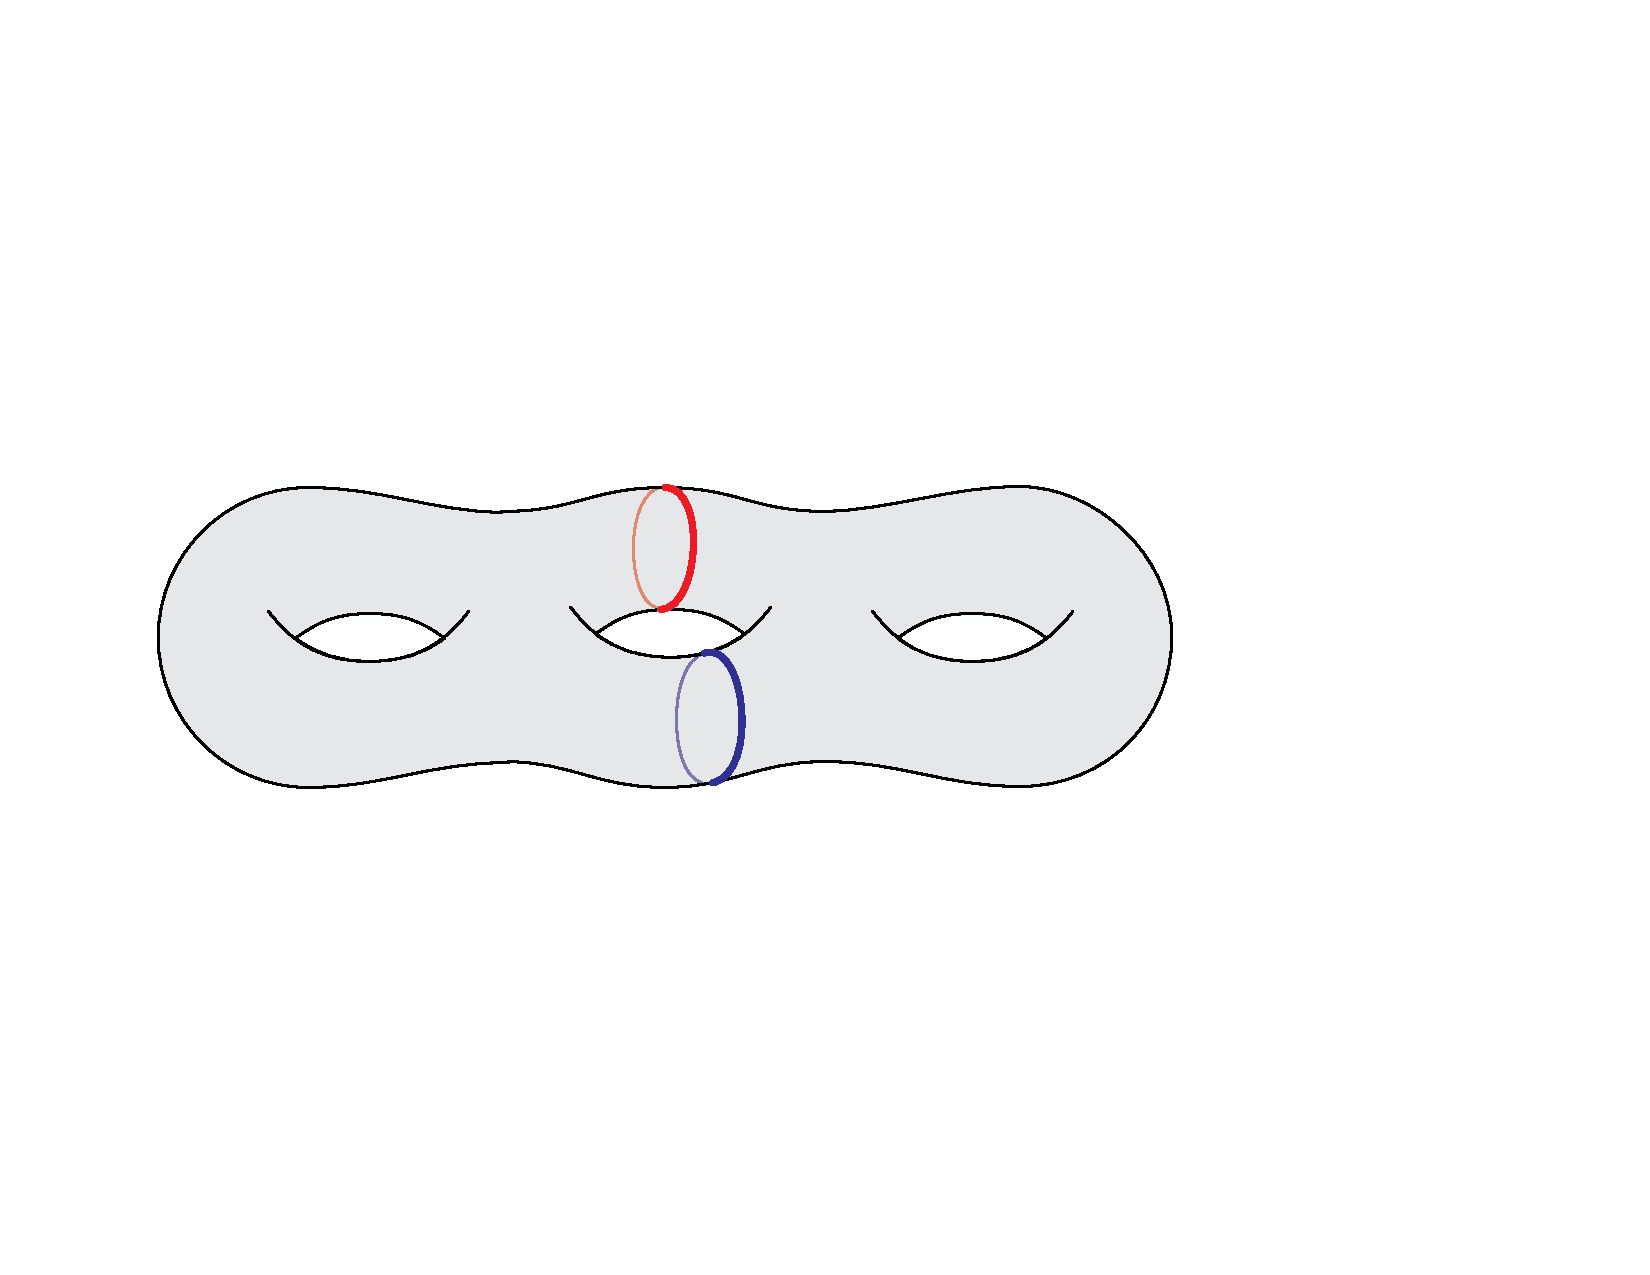
\includegraphics[height=0.75in]{Fig/homologous2}
\caption{Pairs of cycles that are homologous but not homotopic.  (Lighter portions of the curves are on the back side of the surface.)}
\label{F:homology}
\end{figure}

We define the \EMPH{carrier} of a (not necessarily simple) cycle $\cycle$ in~$G$ to be the even subgraph of edges that~$\cycle$ traverses an odd number of times; two cycles are homologous if their carriers are homologous.  A cycle~$\cycle$ is \EMPH{$\Z_2$-minimal} if it has minimum total length among all cycles homologous with $\cycle$.  Similarly, a loop $\ell$ with basepoint~$v$ is $\Z_2$-minimal if it has minimum length among all loops based at $v$ that are homologous with $\ell$.  Every $\Z_2$-minimal cycle can be regarded as a $\Z_2$-minimal loop through any of its vertices.

\fakeparagraph{Covering maps and covering spaces.~}
A continuous map ${\pi \colon \Sigma' \to \Sigma}$ between two surfaces is called a \EMPH{covering map} if each point $x\in \Sigma$ lies in an open neighborhood $U\subset\Sigma$ such that (1)~$\pi^{-1}(U)$ is a countable union of disjoint open sets $U_1\cup U_2\cup\cdots$ and (2)~for each~$i$, the restriction $\pi|_{U_i}:U_i \to U$ is a homeomorphism.  If there is a covering map $\pi$ from $\Sigma'$ to $\Sigma$, we call $\Sigma'$ a \EMPH{covering space} of $\Sigma$.  The \emph{universal cover}~$\widetilde\Sigma$ is the unique simply-connected covering space of $\Sigma$ (up to homeomorphism).  For any path $p$ in $\Sigma$ such that $\pi(x') = p(0)$ for some point $x'\in\Sigma'$, there is a unique path $p'$ in $\Sigma'$, called a \EMPH{lift} of $p$, such that $p'(0) = x'$ and $\pi\circ p'=p$.  Conversely, for any path $p'$ in $\Sigma'$, the path $\pi\circ p'$ is called a \EMPH{projection} of $p'$.

A \emph{deck transformation} for a covering map $\pi\colon \Sigma' \to \Sigma$ is an automorphism $d\colon \Sigma' \to \Sigma'$ such that $\pi\circ d = \pi$; the set of all deck transformations defines a group under composition.  For any normal subgroup $N$ of the fundamental group $\pi_1(\Sigma, x)$, there is a unique path-connected covering space of~$\Sigma$ (up to homeomorphism) whose group of deck transformations is isomorphic to the quotient group $\pi_1(\Sigma, x)/N$.  For example, the universal cover $\widetilde \Sigma$ is the unique path-connected covering space whose deck transformation group is the entire fundamental group $\pi_1(\Sigma, x)$.  The \EMPH{$\Z_2$-homology cover}~$\SIGMABAR$ of $\Sigma$ is the unique path-connected covering space whose group of deck transformations is the first homology group $H_1(\Sigma, \Z_2)$.  We give an equivalent combinatorial definition in the next section.

% --------------------------------------------------------------------------------
\section{Homology Signatures}
\label{S:homology}

Throughout the paper, we fix a directed graph $G=(V,E)$, a non-negative weight function $w\colon E\to \Real$, and a cellular embedding of $G$ on a surface $\Sigma$ of genus $g$ with $b$ boundaries.  Without loss of generality, we assume that the underlying surface $\Sigma$ has at least one boundary; otherwise, we can remove an arbitrary face of $G$ from~$\Sigma$ without affecting its homology at all.  Let $\delta_1, \dots, \delta_b$ denote the boundary cycles of $\Sigma$, and let $\beta = 2g+b-1$ denote the the first Betti number of $\Sigma$.

In this section, we describe a standard method for preprocessing a combinatorial surface in $O(\beta n)$ time, so that the $\Z_2$-homology class of any cycle $\cycle$ can be computed in $O(\beta)$ time per edge.  Our algorithm associates a vector of $\beta$ bits with each edge $e$, called the \EMPH{signature} of~$e$; the homology class of any cycle is characterized by the bit-wise exclusive-or of the signatures of its edges.  These homology signatures are essentially equivalent to the \emph{crossing parity vectors} described by Chambers \etal~\cite{surfcut}, but our construction is slightly more flexible.

Our construction is based on one of two natural generalizations of tree-cotree decompositions~\cite{e-dgteg-03} to surfaces with boundary; the second generalization is introduced in Section \ref{S:cycles}.  We define a \EMPH{tree-coforest decomposition} of $G$ to be any partition $(T, F, X)$ of the edges of $G$ into three edge-disjoint subgraphs with the following properties:
\begin{itemize}\itemsep0pt
\item $T$ is a spanning tree of $G$.
\item $F^*$ is a spanning \emph{forest} of $G^*$, that is, an acyclic subgraph that contains every vertex.
\item Each component of $F^*$ contains a single dual boundary vertex $\delta_i^*$.
\end{itemize}
Euler's formula implies that there are exactly $\beta$ edges in $X$; arbitrarily index these edges $e_1, \dots, e_\beta$.  For each edge $e_i\in X$, adding the corresponding dual edge $e_i^*$ to $F^*$ creates a new dual path $\dualarc_i$, which is either a simple path between distinct boundary vertices, or a nontrivial loop from a boundary vertex back to itself; in the second case, $\dualarc_i$ may traverse some edges of $F^*$ twice.  We can treat each path $\dualarc_i$ as a simple arc in the \emph{abstract} surface $\Sigma$; cutting along these $\beta$ arcs transforms $\Sigma$ into a topological disk.  See Figure \ref{F:tree-coforest}.

\begin{figure}[htb]
\centering\footnotesize\sf
\begin{tabular}{c}
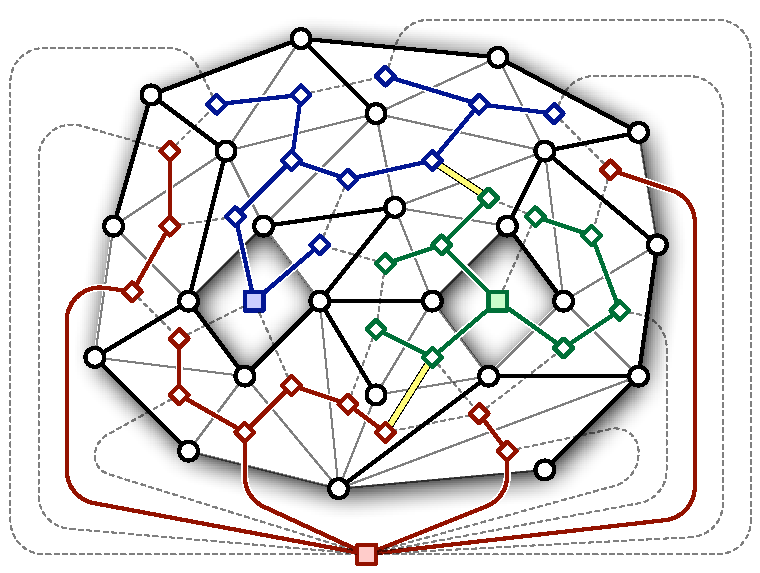
\includegraphics[scale=0.45]{Fig/tree-coforest2} \\
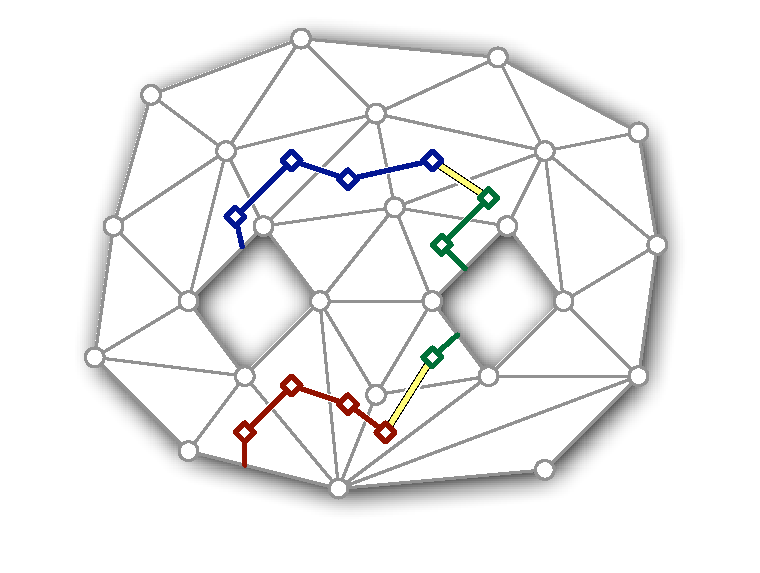
\includegraphics[scale=0.45]{Fig/tree-coforest-arcs2} \\[-3ex]
\end{tabular}
\caption{Top: A tree-coforest decomposition of the graph in Figure~\ref{F:duality}; doubled lines indicate edges in $X$.  Bottom: The resulting system of dual arcs.  Compare with Figure \ref{F:forest-cotree}.}
\label{F:tree-coforest}
\end{figure}

Finally, for each edge $e$ in $G$, we define its signature \EMPH{$[e]$} to be the $\beta$-bit vector whose $i$th bit is equal to $1$ if and only if $e$ crosses $\dualarc_i$ (that is, if $\dualarc_i$ traverses the dual edge $e^*$) exactly once.  The signature $[\eta]$ of an even subgraph $\eta$ is the bitwise exclusive-or of the signatures of its edges.  Similarly, the signature~$[\cycle]$ of a cycle $\cycle$ is the bitwise exclusive-or of the signatures of the edges that $\cycle$ traverses an odd number of times.

Let \EMPH{$h \oplus h'$} denote the bitwise exclusive-or of two homology signatures $h$ and $h'$, or equivalently, their sum as elements of the homology group~$(\Z_2)^\beta$.  The identities $[\eta \oplus \eta'] = [\eta] \oplus [\eta']$ and $[\cycle\cdot\cycle'] = [\cycle] \oplus [\cycle']$ follow directly from the definitions.


\begin{lemma}
\label{L:sign}
We can preprocess $G$ in $O(\beta n)$ time, so that the signature $[\cycle]$ of any cycle can be computed in $O(\beta)$ time per edge.
\end{lemma}

\begin{proof}
A tree-coforest decomposition can be computed in $O(n)$ time as follows.  First construct a graph~$H$ by identifying all the dual boundary vertices in $G^*$ to a single vertex.  Compute a spanning tree of $H$ by whatever-first search; the edges of this spanning tree define an appropriate dual spanning forest~$F^*$.  Construct the subgraph $G\setminus F$ and compute a spanning tree $T$ via whatever-first search.  Finally, let $X = G\setminus (T\cup F)$.  With the decomposition in hand, it is straightforward to compute each path $\dualarc_i$ in $O(n)$ time, and then compute each edge signature in $O(\beta)$ time.
\end{proof}


\begin{figure*}
\centering
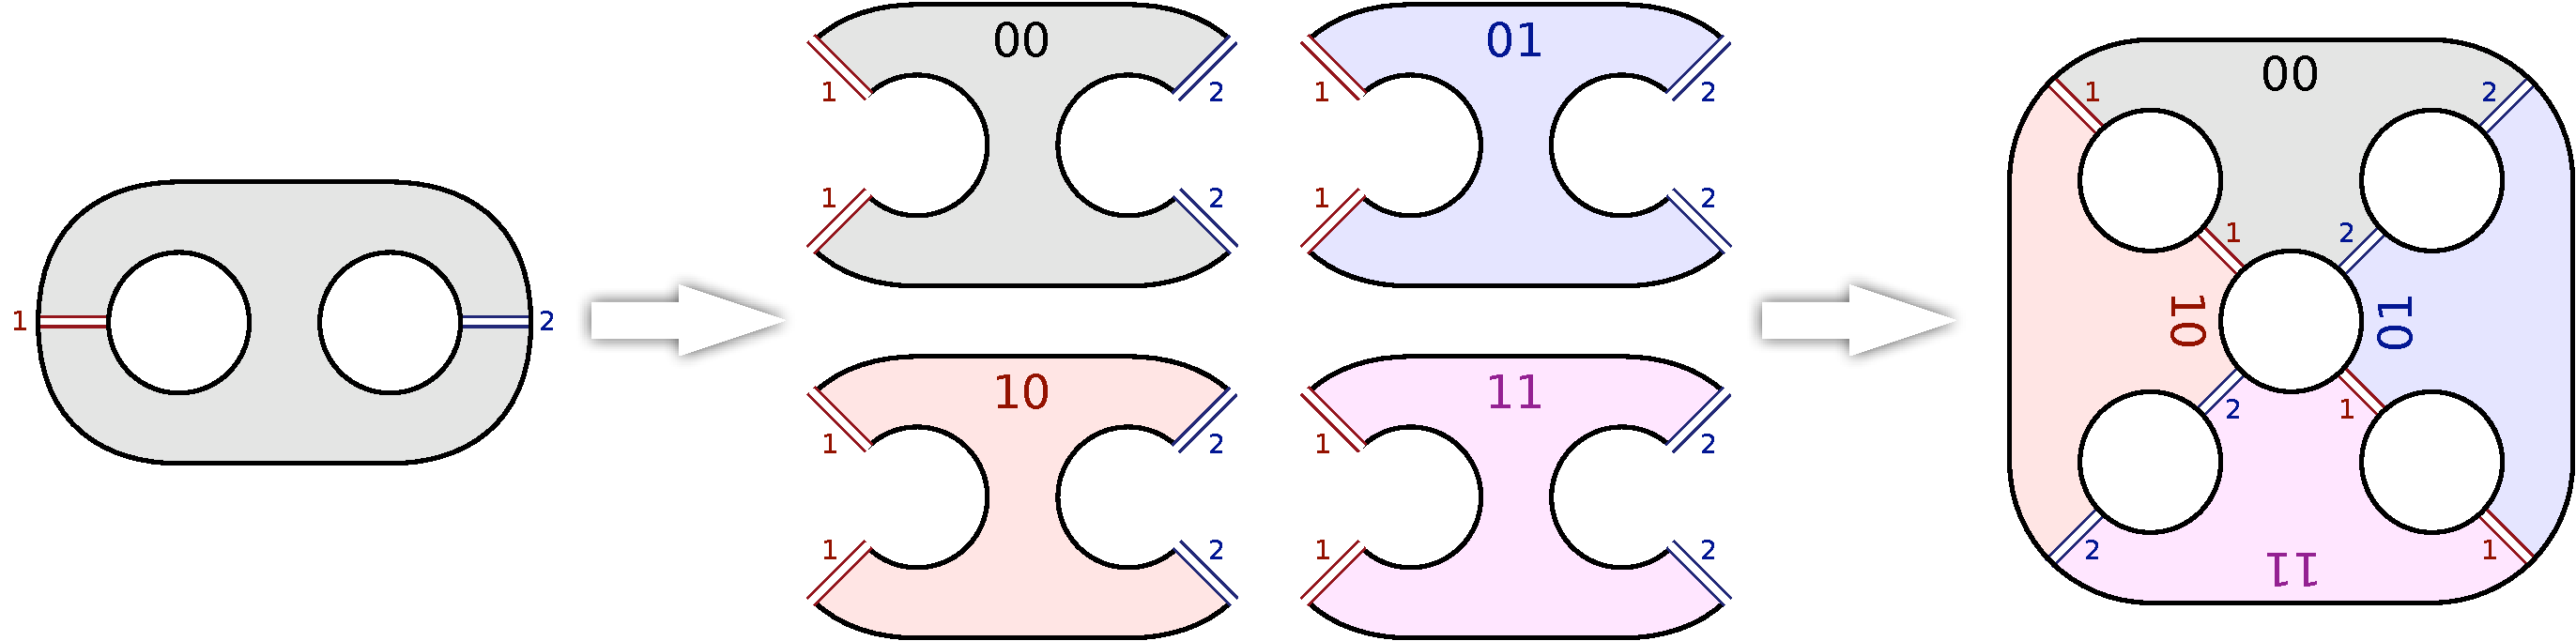
\includegraphics[height=1.5in]{Fig/hom-cover-example}
\caption{Constructing the $\Z_2$-homology cover of a pair of pants (a genus zero surface with three boundaries).}
\label{F:cover-ex}
\end{figure*}



\begin{lemma}
An even subgraph $\eta$ of $G$ is null-homologous in $\Sigma$ if and only if $[\eta] = 0$.
\end{lemma}

\begin{proof}
Let $\eta$ be a null-homologous even subgraph of $G$.  Then by definition, $\eta$ is the boundary of the union of a subset~$Y$ of faces of $G$.  The boundary of any face $f$ is contractible in $\Sigma$ and therefore has signature $0$.  It follows immediately that $[\eta] = [\bigoplus_{f\in Y} \partial f] = \bigoplus_{f\in Y} [\partial f] = 0$.

Conversely, suppose $\eta$ crosses each arc $\dualarc_i$ an even number of times, so $[\eta]=0$.  Let $x$ and $y$ be two intersection points between $\eta$ and some arc $\dualarc_i$, and let $\dualarc_i[x,y]$ be the subpath of $\dualarc_i$ between those two points.  Replacing tiny segments of $\eta$ through~$x$ and~$y$ with two copies of $\dualarc_i[x,y]$ does not change the homology class of $\eta$, but does reduce the number of intersection points between $\eta$ and $\dualarc_i$.  It follows by induction that~$\eta$ is homologous to another even graph $\eta'$ that does not intersect any path~$\dualarc_i$ at all.  This even graph lies entirely within the disk $\Sigma\setminus \bigcup_i\dualarc_i$, and is therefore null-homologous.
\end{proof}


The following corollaries are now immediate.

\begin{corollary}
Two even subgraphs $\eta$ and $\eta'$ of $G$ are $\Z_2$-homologous in $\Sigma$ if and only if $[\eta] = [\eta']$.
\end{corollary}

\begin{corollary}
Two cycles $\cycle$ and $\cycle'$ in $G$ are $\Z_2$-homologous in $\Sigma$ if and only if $[\cycle] = [\cycle']$.
\end{corollary}




% --------------------------------------------------------------------------------
\section{\boldmath The $\Z_2$-Homology Cover}
\label{S:cover}

%Throughout the paper, we fix a directed graph $G=(V,E)$, a non-negative weight function $w\colon E\to \Real$, and a cellular embedding of $G$ on a surface $\Sigma$ of genus $g$ with $b$ boundaries.  Without loss of generality, we assume that the underlying surface $\Sigma$ has at least one boundary; otherwise, we can remove an arbitrary face of~$G$ from~$\Sigma$ without affecting its homology at all.  Let $\delta_1, \dots, \delta_b$ denote the boundary cycles of $\Sigma$, and let $\beta = 2g+b-1$ denote the the first Betti number of $\Sigma$.
%
%In the Appendix, we describe a standard method for preprocessing a combinatorial surface in $O(\beta n)$ time, so that the $\Z_2$-homology class of any cycle $\cycle$ can be computed in $O(\beta)$ time per edge.  Our algorithm associates a vector of $\beta$ bits with each edge $e$, called the \EMPH{homology signature} of $e$ and denoted \EMPH{$[e]$}.  We define the homology signature $[\eta]$ of an even subgraph $\eta$ to be the bitwise exclusive-or of the homology signatures of its edges; similarly, the signature~$[\cycle]$ of a cycle $\cycle$ is the signature of its carrier.  The identities $[\eta \oplus \eta'] = [\eta] \oplus [\eta']$ and $[\cycle\cdot\cycle'] = [\cycle] \oplus [\cycle']$ follow directly from our definitions, where \EMPH{$h \oplus h'$} denotes the bitwise exclusive-or of two homology signatures $h$ and $h'$, or equivalently, their sum as elements of the first homology group~$(\Z_2)^\beta$.

With the homology signatures in hand, the $\Z_2$-homology cover of a combinatorial surface can be defined using a standard~\emph{voltage construction}~\cite[Chapter 4]{gt-tgt-01}, as follows.  Let $\Gbar$ denote the graph whose vertices are all ordered pairs $(v, h)$ where $v$ is a vertex of $G$ and $h$ is an element of $(\Z_2)^\beta$, and whose edges are the ordered pairs $(\arc{u}{v}, h) := (u, h)\arcto(v, h\oplus [u\arcto v])$ for all edges $\arc{u}{v}$ of $G$ and all homology classes $h \in (\Z_2)^\beta$.  Let $\pi\colon \Gbar\to G$ denote the covering map $\pi(v, h) = v$; this map projects any cycle in $\Gbar$ to a cycle in $G$.  To define a cellular embedding of~$\Gbar$, we declare a cycle in $\Gbar$ to be a face if and only if its projection is a face of $G$.  The combinatorial surface defined by this embedding is the $\Z_2$-homology cover $\Sigmabar$.

Our construction can be interpreted more topologically as follows.  Let $\dualarc_1, \dots, \dualarc_\beta$ denote the system of dual arcs used to define the homology signatures $[e]$.  The surface $D := \Sigma\setminus(\dualarc_1\cup\cdots\cup \dualarc_\beta)$ is a topological disk.  Each arc $\dualarc_i$ appears on the boundary of $D$ as two segments $\dualarc^+_i$ and~$\dualarc^-_i$.  For each signature $h\in (\Z_2)^\beta$, we create a disjoint copy $(D,h)$ of $D$; for each index~$i$, let $(\dualarc^+_i, h)$ and $(\dualarc^-_i, h)$ denote the copies of $\dualarc^+_i$ and $\dualarc^-_i$ in the disk $(D, h)$.  For each index~$i$, let~$b_i$ denote the $\beta$-bit vector whose $i$th bit is equal $1$ and whose other $\beta-1$ bits are all equal to~$0$.  The $\Z_2$-homology cover $\Sigmabar$ is constructed by gluing the~$2^\beta$ copies of $D$ together by identifying boundary paths $(\dualarc^+_i,h)$ and $(\dualarc^-_i, h\oplus b_i)$, for every index $i$ and homology class $h$.  See Figure \ref{F:cover-ex} for an example.

\begin{lemma}
\label{L:cover-cxy}
The combinatorial surface $\Sigmabar$ has $\nbar = 2^\beta n$ vertices, genus $\gbar = O(2^\beta \beta)$, and $\bbar = O(2^\beta b)$ boundaries, and it can be constructed in $O(2^\beta n)$ time.
\end{lemma}

\begin{proof}
Let $m$ and $f$ denote the number of edges and faces of $\Sigma$, respectively.  Recall that the Euler characteristic of $\Sigma$ is $\chi = n - m + f = 2 - 2g - b = 1-\beta$.  The combinatorial surface~$\Sigmabar$ has exactly $\nbar = 2^\beta n$ vertices, $2^\beta m$ edges, and $2^\beta f$ faces, so its Euler characteristic is $\chibar = 2^\beta (1-\beta)$.

If $b>1$, then each boundary cycle $\delta_i$ has a non-zero homology signature; at least one arc $\dualarc_j$ has exactly one endpoint on~$\delta_i$.  Thus, $\Sigmabar$ has exactly $\bbar = 2^{\beta-1} b$ boundary cycles, each of which is a double-cover (in fact, the $\Z_2$-homology cover) of some boundary cycle~$\delta_i$.  It follows that~$\Sigmabar$ has genus $\gbar = 1-(\chibar+\bbar)/2 = {2^{\beta-2} ({4g+b-4}) + 1}$.  (Somewhat surprisingly, $\Sigmabar$ may have positive genus even when $\Sigma$ does not!)  On the other hand, when $b=1$, the boundary cycle~$\delta_1$ is null-homologous, so $\Sigmabar$ has $\bbar = 2^\beta b$ boundary cycles, and thus~$\Sigmabar$ has genus $\gbar = {1-(\chibar+\bbar)/2} =  {2^\beta (g-1) + 1}$.

After computing the homology signatures for $\Sigma$ in $O(\beta n)$ time, following Lemma \ref{L:sign}, it is straightforward to construct $\Sigmabar$ in $O(\nbar) = O(2^\beta n)$ time.
\end{proof}

We assign weights to the directed edges of $\Gbar$ by setting $\wbar(\arc{u}{v},h) := w(\arc{u}{v})$ for each edge $\arc{u}{v}$ of~$G$ and each homology class $h$.  In other words, each directed edge in $\Sigmabar$ inherits the weight of its projection in $\Sigma$.

Now consider an arbitrary path $\path$ in $G$, with (possibly equal) endpoints $u$~and $v$.  A straightforward induction argument implies that for any homology class $h \in (\Z_2)^\beta$, the path~$\path$ is the projection of a unique path from $(u,h)$ to $(v,h\oplus[\path])$, which we denote \EMPH{$(\path,h)$}.  Moreover, this lifted path has the same length as its projection: $w(\path) = \wbar(\path,h)$.  The following lemmas are now immediate.

\begin{lemma}
\label{L:lift-shortest}
Every lift of a shortest directed path in $G$ is a shortest directed path in $\Gbar$.
\end{lemma}

\begin{lemma}
\label{L:lift-minimal}
A loop $\ell$ in $G$ with basepoint $v$ is $\Z_2$-minimal if and only if, for every homology class $h\in (\Z_2)^\beta$, the lifted path $(\ell,h)$ is a shortest directed path in $\Gbar$ from $(v,h)$ to $(v,h\oplus[\ell])$.
\end{lemma}

% --------------------------------------------------------------------------------
\section{\boldmath Computing $\Z_2$-Minimal Cycles}
\label{S:cycles}

The results in the previous section immediately suggest imply an algorithm to compute the shortest directed cycle in a given $\Z_2$-homology class $h$ in time $2^{O(\beta)}n^2$: construct the $\Z_2$-homology cover, and then compute the shortest path from $(v,0)$ to $(v,h)$, for every vertex $v$ in the original graph.  In this section, we describe a more complex algorithm that runs in time $2^{O(\beta)}n\log n$.

\begin{lemma}
\label{L:cutpaths}
In $O(n\log n + \beta n)$ time, we can construct a set $S$ of $O(\beta)$ directed shortest paths in~$G$, such that every non-null-homologous cycle in $G$ intersects at least one path in $S$.
\end{lemma}

\begin{proof}
Following Chambers \etal~\cite{splitting}, we construct a \emph{greedy system of arcs}, using a variant of Erickson and Whittlesey's algorithm to construct optimal systems of loops \cite{gohog}.  Our algorithm uses a natural generalization of tree-cotree decompositions~\cite{e-dgteg-03} to surfaces with boundary, essentially dual to the tree-coforest decompositions described in Section \ref{S:homology}.  A \EMPH{forest-cotree decomposition} of $G$ is any partition $(\partial\! G, F, C, X)$ of the edges of $G$ into \emph{four} edge-disjoint subgraphs with the following properties:
\begin{itemize}\itemsep0pt
\item $\partial\! G$ is the set of all boundary edges of $G$.
\item $F$ is a spanning forest of $G$, that is, an acyclic subgraph of $G$ that contains every vertex.
\item Each component of $F$ contains a single boundary vertex.
\item $C^*$ is a spanning tree of $G^*\setminus (\partial G)^*$, that is, a subtree of $G^*$ that contains every vertex \emph{except} the dual boundary vertices $\delta_i^*$.
\end{itemize}
Euler's formula implies that there are exactly $\beta$ edges in $X$; arbitrarily label these edges $e_1, e_2, \dots, e_\beta$.  For each edge $e_i\in X$, the subgraph~$F\cup \set{e_i}$ contains a single nontrivial arc $\primalarc_i$, which is either a simple path between distinct boundary cycles, or a nontrivial loop from a boundary cycle back to itself; in the second case, $\primalarc_i$ may traverse some edges of $F$ twice.  Cutting along the arcs $\primalarc_1, \dots, \primalarc_\beta$ transforms~$\Sigma$ into a topological disk.  Thus, every non-null-homologous cycle in $G$ must cross at least one arc~$\primalarc_i$.   See Figure \ref{F:forest-cotree}.

\begin{figure}[htb]
\centering\footnotesize\sf
\begin{tabular}{c}
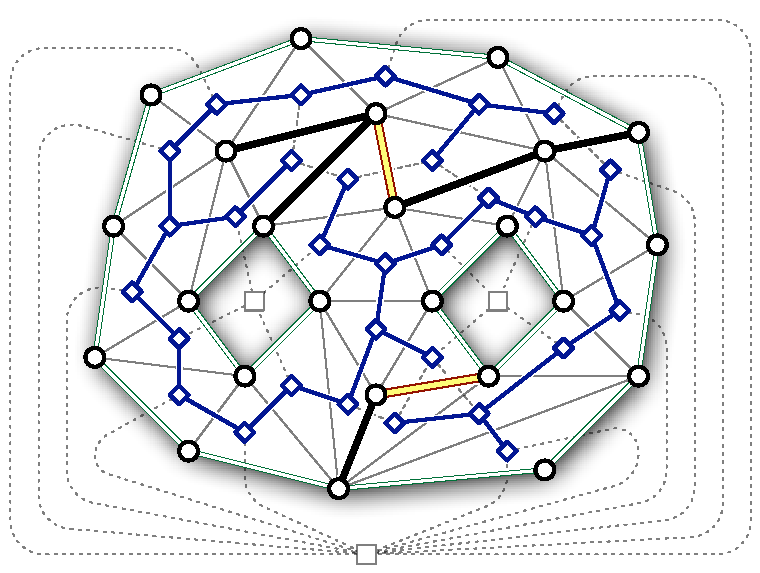
\includegraphics[scale=0.45]{Fig/forest-cotree2} \\
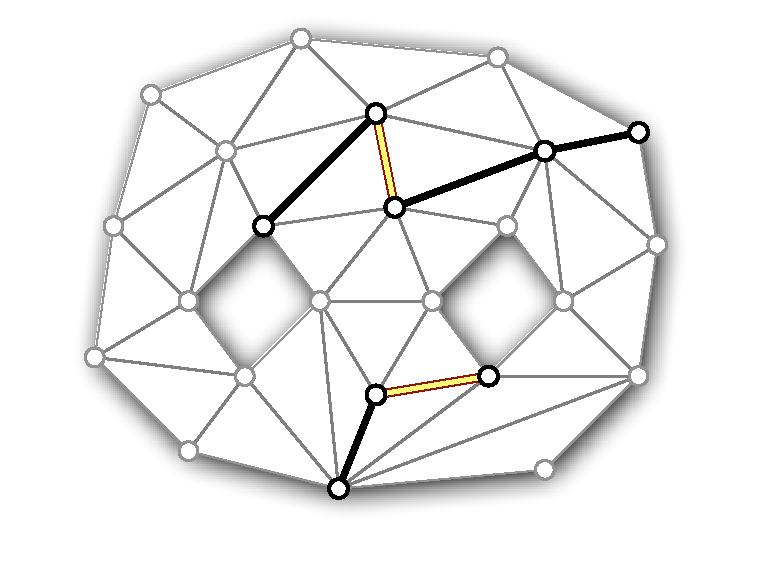
\includegraphics[scale=0.45]{Fig/forest-cotree-arcs2} \\[-3ex]
\end{tabular}
\caption{Top: A forest-cotree decomposition of the graph in Figure \ref{F:duality}; thick doubled lines indicate edges in $X$.  Bottom: The resulting system of arcs.  Compare with Figure \ref{F:tree-coforest}.}
\label{F:forest-cotree}
\end{figure}

We can easily construct an \emph{arbitrary} forest-cotree decomposition in $O(n)$ time using whatever-first search, as in Lemma \ref{L:sign}, but we require a decomposition with a particular forest $F$.  Let $G/\partial G$ denote the graph obtained from $G$ by \emph{contracting} the entire subgraph $\partial G$---both vertices and edges---to a single vertex $x$.  Using Dijkstra's algorithm, we compute the single-source shortest-path tree $T$ in $G/\partial G$ rooted at $x$ in $O(n\log n)$ time.  Let $F$ be the subgraph of $G$ corresponding to~$T$.  Each component of $F$ is a tree of shortest paths from a boundary vertex to a subset of the non-boundary vertices of $G$.  With the shortest-path forest $F$ in hand, we can easily construct the rest of the forest-cotree decomposition in $O(n)$ time.

Finally, for each edge $e_i\in X$, let $\sigma_i$ and $\tau_i$ denote the unique directed paths in $F$ from the boundary of~$G$ to the endpoints of $e_i$, and let $S := \set{\sigma\!_1, \dots, \sigma\!_\beta, \allowbreak \tau_1, \dots, \tau_\beta}$.  By construction of $F$, every element of~$S$ is a (possibly empty) shortest directed path.  Moreover, because $\primalarc_i = \sigma_i \cdot e_i \cdot \rev(\tau_i)$ for each index $i$, every non-null-homologous cycle in $G$ must intersect at least one path in $S$.  We can easily compute each path in $S$ in $O(n)$ time.
\end{proof}

Recall that any path $\sigma$ from $u$ to $v$ in $G$ is the projection of a unique path $(\sigma,0)$ from $(u,0)$ to $(v,[\sigma])$ in $\Gbar$.

\begin{lemma}
\label{L:nocross}
Let $\cycle$ be a $\Z_2$-minimal cycle in $G$, and let~$\sigma$ be any shortest path in $G$ that intersects $\cycle$.  There is a $\Z_2$-minimal cycle $\cycle'$ homologous to $\cycle$, which is the projection of a shortest path $(\cycle', h)$ in $\Gbar$ that starts with a subpath of $(\sigma, 0)$ but does not otherwise intersect $(\sigma, 0)$.
\end{lemma}

\begin{proof}
Let $v$ be the vertex of $\sigma\cap\cycle$ closest to the starting vertex of $\sigma$, and let $(v,h)$ be the corresponding vertex of the lifted path $(\sigma,0)$.  Think of~$\cycle$ as a loop based at $v$.  Lemma \ref{L:lift-minimal} implies that the lifted path $(\cycle, h)$ is a shortest path from $(v,h)$ to $(v,h\oplus [\cycle])$.

Now let $(w,h')$ be the last vertex along $(\cycle,h)$ that is also a vertex of $(\sigma,0)$.  Let $(\cycle', h)$ be the path obtained from $(\cycle, h)$ by replacing the subpath from from $(v,h)$ to $(w,h')$ with the corresponding subpath of $(\sigma,0)$.  By construction, $(\cycle', h)$ starts with a directed subpath of $(\sigma,0)$ but does not otherwise intersect $(\sigma,0)$.   Because both $(\cycle, h)$ and $(\sigma,0)$ are shortest paths in $\Sigmabar$, the new path $(\cycle', h)$ has the same length as $(\cycle, h)$.  Thus, the projected cycle $\cycle'$ has the same length and homology class as $\cycle$, which implies that~$\cycle'$ is $\Z_2$-minimal.
\end{proof}

We emphasize that the modified cycle $\cycle'$ may intersect~$\sigma$ arbitrarily many times; however, all such intersections lift to intersections between $(\cycle', h)$ and lifts of $\sigma$ other than $(\sigma, 0)$.

Our algorithm uses a recent generalization of Klein's seminal multiple-source shortest path algorithm~\cite{k-msspp-05} to higher-genus embedded graphs:

\begin{lemma}[Chambers \etal~\cite{cc-msspg-07,multishort}]
\label{L:multishort}
Let $G$ be a directed graph with non-negative edge weights, cellularly embedded on a surface $\Sigma$ of genus $g$ with $b>0$ boundaries, and let $f$ be an arbitrary face of $G$.  We can preprocess $G$ in $O(gn\log n)$ time\,\footnote{The published version of this algorithm \cite{cc-msspg-07} proves a weaker time bound of $O(g^2n\log n)$; using this version increases the running time of our algorithms by a factor of $2^\beta$.}\! and $O(n)$ space, so that the length of the shortest path from any vertex incident to $f$ to any other vertex can be retrieved in $O(\log n)$ time.
\end{lemma}

\begin{theorem}
\label{Th:min-cycle}
Let $G$ be a directed graph with non-negative edge weights, cellularly embedded on a surface~$\Sigma$ with first Betti number $\beta$, and let~$\cycle$ be a cycle in~$G$ with $k$ edges.  A shortest directed cycle in~$\Sigma$ that is $\Z_2$-homologous with~$\cycle$ can be computed in $O(\beta k + 4^\beta \beta^2\, n\log n)$ time.
\end{theorem}

\begin{proof}
We begin by computing homology signatures for the edges of $G$ in $O(\beta n)$ time, as described in Section~\ref{S:homology}.  In $O(\beta k)$ time, we then compute the homology signature~$[\cycle]$.  If $[\cycle] = 0$, we return the empty walk and halt.

Next, we construct the $\Z_2$-homology cover $\Gbar$ in $O(2^\beta n\log n)$ time, as described in Section~\ref{S:cover}, as well as the set $S$ of directed shortest paths described in Lemma~\ref{L:cutpaths}.  We then look for the shortest path in $\Gbar$ of the canonical form described in Lemma~\ref{L:nocross}, by considering each shortest path $\sigma\in S$ in turn as follows.

Let us write $(\sigma,0) = (v_0,0) \arcto (v_1,h_1) \arcto\allowbreak \cdots\arcto (v_t, h_t)$.  We construct the combinatorial surface $\Sigmabar\snip(\sigma,0)$ by splitting the path $(\sigma,0)$ into two parallel paths from $(v_0,0)$ to $(v_t,h_t)$, which we denote  $(\sigma,0)^+$ and $(\sigma,0)^-$.  For each index $1\le i\le t-1$, let $(v_i,h_i)^+$ and $(v_i,h_i)^-$ denote the copies of vertex $(v_i,h_i)$  on the paths $(\sigma,0)^+$ and $(\sigma,0)^-$, respectively.  The paths $(\sigma,0)^+$ and $(\sigma,0)^-$ bound a new common face $f_{(\sigma,0)}$ in $\Sigmabar\snip(\sigma,0)$.

Lemma \ref{L:nocross} implies that if any $\Z_2$-minimal cycle homologous to $\cycle$ intersects $\sigma$, then some $\Z_2$-minimal cycle homologous to $\cycle$ is the projection of a shortest path in $\Sigmabar\snip(\sigma,0)$ from some vertex $(v_i,h_i)^\pm$ to the corresponding vertex $(v_i, h_i\oplus[\cycle])$.  To compute these shortest paths, we implicitly compute the shortest path in $\Sigmabar\snip(\sigma,0)$ from every vertex on the boundary of $f_{(\sigma,0)}$ to \emph{every} vertex of $\Sigmabar\snip(\sigma,0)$, using Lemma~\ref{L:multishort}.  The resulting algorithm runs in $O(\gbar\,\nbar \log \nbar) = O(4^\beta \beta^2\, n\log n)$ time, by Lemma \ref{L:cover-cxy}.
\end{proof}

By running this algorithm $2^\beta$ times, we can compute the shortest directed cycle in $\Sigma$ in \emph{every} $\Z_2$-homology class, in $O(8^\beta \beta^2\, n\log n)$ time.  In particular, we can compute the shortest directed cycle in~$\Sigma$ that has nontrivial $\Z_2$-homology.  When the original surface has no boundary, this is just the shortest \emph{non-separating} cycle in $\Sigma$.  Very recently, Cabello \etal~\cite{ccl-fsncd-10} described an algorithm to compute the shortest non-separating cycle in any surface-embedded directed graph in $O(g^{1/2} n^{3/2}\log n)$ time; our new algorithm is faster whenever $g \le (\lg n)/13$.

\begin{corollary}
\label{C:nonsep}
Given a directed graph $G$ with $n$ vertices with non-negative edge weights, cellularly embedded on a surface with genus~$g$, we can compute the shortest directed cycle in $G$ that is non-separating in $\Sigma$ in $O(64^g g^2 n\log n)$ time.
\end{corollary}

Cabello \etal~\cite{ccl-fsncd-10} also described an algorithm to find the shortest \emph{non-contractible} cycle in an embedded directed graph in $O(g^{1/2} n^{3/2}\log n)$ time.  Our approach does not lead to a faster algorithm for this problem;  contractibility is inherently  a property of \emph{homotopy}, not homology.

% --------------------------------------------------------------------------------
\section{Faster Minimum Cuts}
\label{S:mincut}

We now apply our algorithm for computing $\Z_2$-minimal cycles to the classical minimum cut problem for \emph{undirected} surface-embedded graphs.  Our approach is motivated by the following lemma of Chambers~\etal~\cite[Lemma 3.1]{surfcut}:

\begin{lemma}
\label{L:mincut-z2}
Let $H$ be an undirected graph with non-negative edge capacities, embedded on a surface~$\Pi$ without boundary, and let $s$ and $t$ be vertices of~$H$.  Finally, let $X$ be the minimum-capacity $(s,t)$-cut in~$H$.  Then~$X^*$ is the minimum-weight even subgraph of $H^*$ that is $\Z_2$-homologous with the boundary of~$s^*$ in the surface $\Pi\setminus(s^*\cup t^*)$.
\end{lemma}

We must emphasize that this characterization applies only to \emph{undirected} graphs, or equivalently, symmetric directed graphs where the capacity of any edge is equal to the capacity of its reversal.  Even for directed \emph{planar} graphs, where the dual of the minimum cut is a simple cycle, the characterisation is incorrect: The minimum-weight cycle $\Z_2$-homologous to $\partial s^*$ in the annulus $\Pi\setminus(s^*\cup t^*)$ is either the dual of the minimum $(s,t)$-cut \emph{or the dual of the minimum $(t,s)$-cut}.  (Of course, if the graph $H$ is undirected, the minimum $(s,t)$-cut and the minimum $(t,s)$-cut coincide.)

\medskip
Like Chambers~\etal~\cite{surfcut}, we actually describe an algorithm to compute the minimum-weight even subgraph in \emph{every} $\Z_2$-homology class.  Theorem \ref{Th:min-cycle} immediately implies that we can compute a minimum-weight \emph{cycle} in every $\Z_2$-homology class in $O(8^\beta \beta^2\, n\log n)$ time.  However, the minimum weight \emph{even subgraph} in a given homology class may not be (the carrier of) a $\Z_2$-minimal cycle.  In particular, if a $\Z_2$-minimal cycle $\gamma$ traverses any edge more than once, then every minimum-weight even subgraph with signature $[\gamma]$ \emph{must} be disconnected.

However, any \emph{connected} $\Z_2$-minimal even subgraph is the carrier of a $\Z_2$-minimal cycle, and the components of any $\Z_2$-minimal even subgraph are themselves $\Z_2$-minimal even subgraphs.  Thus, we can assemble a $\Z_2$-minimal even subgraph in any homology class from a subset of the $\Z_2$-minimal cycles we have already computed.  The following lemma puts an upper bound on the number of cycles we need.

\begin{lemma}
\label{L:even-comps}
Every $\Z_2$-minimal even subgraph of $G$ has at most $g+b-1$ components.
\end{lemma}

\begin{proof}
Let $\gamma_1, \dots, \gamma_{g+b}$ be disjoint simple cycles on an \emph{abstract} surface $\Sigma$ of genus $g$ with $b$ boundaries, and consider the surface $\Sigma' = \Sigma \setminus (\gamma_1 \cup \cdots \cup \gamma_{g+b})$.  The definition of genus implies that $\Sigma'$ cannot be connected; indeed, $\Sigma'$ must have at least $b+1$ components.  So the pigeonhole principle implies that some component $\Sigma''$ of~$\Sigma$ does not contain any of the boundary cycles of $\Sigma$.  The boundary of $\Sigma''$ is therefore null-homologous.

Following Chambers \etal~\cite{surfcut}, call a cycle in $G$ \emph{weakly simple} if it traverses each edge of $G$ at most once and never crosses itself.  Any weakly simple cycle in $G$ can be perturbed into a simple cycle in an arbitrarily small neighborhood of $G$.  A \emph{cycle decomposition} of an even subgraph $\eta$ is a set of edge-disjoint, non-crossing, weakly simple cycles whose union is $\eta$.  It is easy to prove that every even subgraph has a cycle decomposition~\cite[Lemma 3.2]{surfcut}.

Now let $\eta$ be an even subgraph of $G$ with more than $g+b-1$ components.  Each component has a cycle decomposition, so $\eta$ must have a cycle decomposition with more than $g+b-1$ elements.  Thus, the argument in the first paragraph implies that some subgraph of $\eta$ must be null-homologous.  We conclude that $\eta$ is not $\Z_2$-minimal.
\end{proof}

\begin{theorem}
\label{Th:min-even}
Let $G$ be an \textbf{undirected} graph with non-negative edge weights, cellularly embedded on a surface~$\Sigma$ with first Betti number $\beta$.  A minimum-weight even subgraph of $G$ in each $\Z_2$-homology class can be computed in $O(8^\beta \beta^2\, n\log n)$ time.
\end{theorem}

\begin{proof}
Our algorithm computes a minimum-weight cycle~$\gamma_h$ in every $\Z_2$-homology class~$h$ in $O(8^\beta \beta^2\, n\log n)$ time, via Theorem \ref{Th:min-cycle}, and then assemble these $\Z_2$-minimal cycles into $\Z_2$-minimal even subgraphs using dynamic programming.

For each homology class $h\in (\Z_2)^\beta$ and each integer $1\le k\le g+b-1$, let \EMPH{$C(h,k)$} denote the minimum total weight of any set of at most $k$ cycles in $G$ whose homology classes sum to $h$.  Lemma~\ref{L:even-comps} implies that the minimum weight of any even subgraph in homology class~$h$ is exactly $C(h, g+b-1)$.  This function obeys the following straightforward recurrence:
\[
	C(h,k) = \min\Setbar{C(h_1,k-1) + C(h_2, 1)}{h_1\oplus h_2 = h}.
\]
This recurrence has two base cases: $C(0, k) = 0$ for any integer $k$, and for any homology class $h$, the value $C(h,1)$ is just the length of $\gamma_h$.  A standard dynamic programming algorithm computes $C(h, g+b-1)$ for all $2^\beta$ homology classes $h$ in $O(4^\beta \beta)$ time.  We can then assemble the actual minimum-weight even subgraphs in each homology class in $O(\beta n)$ time.  The total time for this phase of the algorithm is $O(4^\beta \beta + 2^\beta \beta n)$, which is dominated by the time to compute all the $\Z_2$-minimal cycles.
\end{proof}

Lemma \ref{L:mincut-z2} and Theorem~\ref{Th:min-even} immediately give us the following result:

\begin{corollary}
\label{C:mincut}
Given an undirected graph $H$ with non-negative edge capacities, embedded on a surface~$\Sigma$ with genus $g$, and two vertices let $s$ and $t$, we can compute a  minimum $(s,t)$-cut in $H$ in $O(16^g g^2 n\log n)$ time.
\end{corollary}


\bibliographystyle{newabuser}
\bibliography{jeffe,topology,data-structures,optimization,homcover-misc}

% --------------------------------------------------------------------------------
%\section*{Appendix: Omitted Proofs}
%\label{S:appendix}

\end{document}

